\documentclass[Journal, InsideFigs, DoubleSpace]{ascelike} %NewProceedings, Journal

%include package for inserting picture
\usepackage{graphicx}%insert image
\DeclareGraphicsExtensions{.pdf,.png,.jpg}
\graphicspath{{figures/}}%folder contains images

\usepackage{caption}%packages for inserting multiple pictures
\usepackage{subcaption}%packages for inserting multiple pictures

\usepackage{array}%for table with fixed width
\newcolumntype{L}[1]{>{\raggedright\let\newline\\\arraybackslash\hspace{0pt}}m{#1}}
\newcolumntype{C}[1]{>{\centering\let\newline\\\arraybackslash\hspace{0pt}}m{#1}}
\newcolumntype{R}[1]{>{\raggedleft\let\newline\\\arraybackslash\hspace{0pt}}m{#1}}

\usepackage{amsmath} %math package

\usepackage{algorithm} %algorithm package
\usepackage[noend]{algpseudocode} % pseudo code package

\usepackage[utf8]{inputenc}%french accents
\usepackage[T1]{fontenc} %for accented characters

\usepackage{booktabs}%allowing drawing hline in table crossing only some columns


\begin{document}

\title{InfraLex: An automatically-generated infrastructure lexicon for matching data entities and attributes from heterogeneous sources}
%TODO: distinguish between lexicon, thesarus and ontology
%
\author{
Tuyen Le
\thanks{
Ph.D. Student, Department of Civil, Construction and Environmental Engineering, Iowa State University. Ames, IA 50011, United States. E-mail: ttle@iastate.edu.},
\and
H. David Jeong
\thanks{Associate Professor, Department of Civil, Construction and Environmental Engineering, Iowa State University. Ames, IA 50011, United States. E-mail: djeong@iastate.edu.}
 }

\maketitle
%
\begin{center}
(To be submitted to the Journal of Computing in Civil Engineering) 
\end{center}

\begin{abstract} %150-175 words (as required by ASCE)
%background:
The inconsistency of data terminology due to the fragmented nature of the civil industry has imposed big challenges for integrating life-cycle digital data from distinct sources to support decision making in highway asset management. The issue of data ambiguity may lead to the lack of common understanding to the same data between the data sender and receiver. While the aspect of data structure has been well addressed thanks to the availability of various international neutral data standards such as LandXML and TransXML;  the semantic aspect still has been neglected by researchers. 
%research objective
This paper presents a novel methodology to construct an automatically-generated lexicon which is consisted of commonly used technical terms for civil infrastructure projects. The lexicon provides an underlying resource for computational systems that perform semantics analysis in the civil infrastructure domain.
%research methods
Natural Language Processing (NLP) techniques and the C-value method are used to detect technical terms from a highway text corpus collected from roadway design guidelines across the U.S. A model for measuring term similarity is trained using the Skip-gram model which uses the corpus as the training dataset. This semantic model is then utilized by a term classification algorithm to organize related terms into separate groups according to their semantic relations.
%result
The developed lexicon has been experimented on the ability of recognizing the most semantically similar terms and achieved a precision of 80 percent. 
  
\end{abstract}

\KeyWords{Civil infrastructure project, Lexicon, Data retrieval, Natural language interface, NLP, Vector space model}
%
%\newpage


%********************************************************
%good terms and phrases:

%adj: nonhierarchical, superior, well-defined; foreseeable; rigid, flexible, empirical, disparate, isolated, 

%sentence strucutre:  this is evidenced by the accelerating emergence of ...; 

%noun: challenges, barrier, hinders, obstacles, impediment; that approximate concepts; extraction=deduction=acquisition; broad spectrum; overtake these technical and economic challenges; bottleneck; data crreation and utilization; in the midst of planning; interpretation; 

%verb: emcombass; tackle, foster, amplified; simplified; detect; aggregate; 

%sentence template: tailored with respect to their context; includes three phases, namely AA, BB and CC; at such places as parks, fairgounds or town spuares; case-specific developments; area of interests; incrementally built; inexpensive and easy-to-use testing device; time and cost-efficient way; research community; one of..since then is the; RDF structure..to make assertion about a resource; syntax-centered NLP;  such as A, B, etc.; ..is in it's reliance upon the presence..which is..; with the objectives of disambiguation; has triggered a mounting awareness; to be the main impediment to the progess; ..start point for deducing other truth; lastly; there is a large body of research on; see e.g. [2], [14] and [32]; the former, the latter; rigorously formalized; backbone strucutre of st; was opted to; Sections 4.5 and 4.6; (e.g., Neo4J, OrientDB, Titan); forthcoming year; well-designed process; is subject to do st; in turn means that; discussion by academics and professionals; some insights on planning, management, and control; strategic framework; in-depth project performance; in lieu of; 

%term': empirical work; linguistic unit/term; 

%axiomatic richness, formality of representation,  

%the following expression denotes, is presented/defined as follows, this/below example shows, the snippet below presents, the following is the short description of the rule, an OWL ontology describing an ifcwindow class, these concepts and relationships can be encoded in the following RDF/XML fragment, is written in Turtle syntax/format:
%The tool is meant to assess, 
%********************************************************

\section{Introduction}%900 words
%Topic introduction, territory: centrality--> genearal background information 
%the background of data extraction
%
The implementation of advanced computerized technologies such as 3D modeling and Geographic Information System (GIS) throughout the life cycle of a civil infrastructure project has allowed a large portion of project data to be available in digital format. The efficiency improvement in sharing these data between project participants and stages, will in turn, translates into increased productivity, efficiency in project delivery and accountability. However, a highway asset as a whole has not yet fully benefited from the potentials of digital models as an accessible, reusable and reliable information source for life-cycle decision making. According to a study conducted by the National Institute of Standard and Technology (NIST), the un-interoperability issue was reported to cost the U.S. capital facilities industry at least \$15.8 billion per year, and two-thirds of those costs were incurred during the operation and maintenance stages \cite{Gallaher04}. The major cost was time spent finding, verifying, and transferring facility and project information into a useful format. This finding indicates that the lack of readiness for downstream phases to directly use the transferred digital project data generated from upstream design and construction stages results in high operational costs.
\par
Due to the fragmented nature of the construction industry, data terminology varies between phases, stakeholders, or geographic regions (counties, states, etc.). Polysemy and synonymy are two major semantic obstacles to the integration and use of data from multiple sources. Polysemy refers to cases when a unique term has distinct meanings. For example, the term 'roadway type', in a generic context, can mean the classification of roadways in terms of either material, function or location; but in the highway context, it refers to roadway functional classification. In contrast, synonymy is associated with the diversity of terms for the same concept. For instance, the longitudinal centerline of a roadway has various terms including 'profile', 'crest', 'grade-line' and 'vertical alignment'. Simply mapping of data names will likely lead to the failure or improper extraction of the desired data. Thus, addressing the terminology ambiguity issue becomes critical to ensure the common understanding on the same dataset between software applications and guarantee the extraction of right data and proper integration of data from multiple sources.
\par
%niche: the importance of dictionaries, ontologies to text analysis, mining and the shortage of dictionaries in civil industry
Research to address the issue of terminology inconsistency in the construction industry is limited. Due to this reason, although an extensive amount of research effort has been made for last several decades in standardizing a neutral data format, such as Industry Foundation Classes (IFC) \cite{buildingsmartIFC} or LandXML \cite{landxml15}, the vision of seamless exchange of data is still in slow progress. One of the approach to enable proper and ambiguity-free reuse of digital data is to develop Model View Definitions (MVD) \cite{buildingSmart} which formally identifies a mapping matrix between the data entities in a neutral data format and the local domain data labels for a specific transaction scenario. MVD enables partial models to be easily extracted and unambiguously interpreted. However, this approach is on a case-by-case and manual basis, and takes years to be completed and maintained; there is demand for more rigorous computational techniques that can allow for automated extraction of data with minimized human interfere \cite{venugopal12,eastman12}. In addition to MVD, a few construction domain specific semantic resources have been proposed, for example the Civil Engineering Thesaurus (CET) \cite{abuzir02}, e-Cognos \cite{wetherill02}, and buildingSMART data dictionary (ISO 12006-3) \cite{buildingsmartData}. These knowledge bases present domain concepts in machine-readable format and allow computer systems to understand meanings of terms. Thus, data mismatch when unifying isolated data sources would be eliminated. They, however, are mainly hand-coded. Due to this reason, the existing domain digital dictionaries still cover only a small portion of the civil infrastructure related concepts. Therefore, there is a demand for computational techniques that can automatically construct and maintain these digital dictionaries to keep up with the increasingly arising of new terms. 
%Identify the niche: overall to one aspect to be addressed--> limitation in current state -->highlight the problem, raise general questions, propose general hypotheses --> emphasize the need (justify the need to address)
\par
% potential tools and method to address the above issue
Recent achievements in accuracy and processing time of advanced Natural Language Processing (NLP) techniques which employ statistics and machine learning have driven text mining and cognitive recognition research to a new era. There is a rich set of NLP tools supporting text processing ranging from for single linguistic units such as Part of Speech (POS) tagging \cite{Toutanova03,Cunningham02}, to relationships between linguistic units like dependency parser \cite{chen14}. These basic NLP techniques have been applied in various computational methods that can support linguistic analysis at the semantic level of terms such as Word2vec \cite{mikolov13a}, and Glove \cite{pennington2014glove}. The availability of these NLP tools offers considerable potentials for the construction industry where most of the domain knowledge resources are in text documents (e.g., design guidelines, specifications, etc.). The implementation of NLP will allow a fast translation of domain knowledge into computer-readable format which is required for a machine-to-machine based data exchange.
\par
%Objectives (research goals, questions/hypotheses, methodology, and main results) --> claiming the value of the research --> outline the structure of the paper
This paper presents the process of translating text based domain knowledge into InfraLex, an extensive civil engineering machine-readable dictionary of technical terms. In order to achieve that goal, basic Natural Language Processing (NLP) techniques and the C-value method \cite{frantzi20} are used to detect technical terms from a highway text corpus collected from roadway design guidelines across the U.S. A model for measuring term similarity is trained using the Skip-gram model \cite{mikolov13a} which uses the highway corpus as the training dataset. This semantic model is then utilized by a proposed term classification algorithm to organize related terms into separate groups according to their semantic relations. The framework was complied into a Java package and a lexicon dataset which can be found at https://github.com/tuyenbk/mvdgenerator.
%
\par
The paper is organized as follows. This section presents background and rationale for the study. Section \ref{sec:litrev} provides underling knowledge supporting the study and gap of knowledge. Section \ref{sec:infralex} and \ref{sec:infralex} respectively describes the methodology employed to develop InfraLex and the performance evaluate results. Research limitations and potential applications will be discussed in Section \ref{sec:dis}. The final section concludes the paper with the discussion on major findings and future research.
% 
\section{Related research} \label{sec:litrev} %2000 words
%section introduction
This section will first present the state-of-the-art regarding NLP and methods to measure semantic similarity which is followed by a review of related research and the gap of knowledge associated with data disambiguation in the civil infrastructure sector.
%
\subsection{Natural Language Processing}
%what is natural languange processing
NLP is a collection of techniques that can analyze and extract information from natural languages like text and speech. The major applications of NLP include translation, information extraction, opinion mining \cite{Cambria14}. These applications are embodied by a rich set of NLP techniques ranging from syntactic  processing at the word individual level such as Tokenization (breaking a sentence into individual tokens) \cite{Webster92,Zhao11},  Part-of-Speech (POS) tagging (assigning tags like adjective, noun, verb, etc. to each token of a sentence) \cite{Toutanova03,Cunningham02}, and Dependency parser (relationships between linguistic units) \cite{chen14},  to semantic level like word sense disambiguation \cite{Lesk86,Yarowsky95,Navigli09}, etc. NLP methods can be classified into two main groups: (1) rule-based and (2) machine-learning (ML) based methods. Rule-based methods, which rely solely on hand-coded rules, are not able to fully cover all complicated sets of human grammatical rules \cite{Marcus95}; and their performance are therefore relatively low. NLP research is shifting to statistical ML-based methods \cite{Cambria14}. ML models are able to accurately learn patterns from training examples to predict the output. Hence, they are independent of languages and linguistic grammars \cite{costa-jussa12}.
%
\subsection{Vector space model}
%
Measuring semantic similarity between semantic units (words, phrases, sentences, concepts, etc.)  is one of the main NLP-related research topics. There are two major approaches for semantic measure including (1) dictionary-based method and (2) distributional method \cite{harispe13}.  The former method relies on a digital dictionary that consists of terms organized in a lexical hierarchy of semantic relations such as synonym, attribute, hypernym/hyponym, etc. Computational platforms (e.g., information retrieval) built upon such dictionaries are able to fast measure the semantic similarity by computing the distances between words in the hierarchy. Hence, this method would be an ideal solution when digital dictionaries are available. However, digital dictionaries are typically hand-crafted; they are therefore not available to many domains \cite{kolb08}. The latter major method for estimating word similarity is based on the distributional model which represents meanings of words through their contexts (surrounding words) in the corpus \cite{erk12}. A distributional model stands on the distributional hypothesis that states that two similar terms would occur in the same context \cite{Harris54}. The outcome of this approach is a Vector Space Model (VSM), in which each vector depends on the co-occurrence frequencies between the target word with other words in the vocabulary. The similarity between semantic units in this model is represented by the distance between corresponding points \cite{erk12}. VSM outperforms the dictionary-based method in terms of time saving as the semantic model can be automatically obtained from text corpus and corpus collecting is much easier than manually constructing a digital dictionary \cite{turney10}. Among the methods to develop VSM, Skip-Gram model \cite{mikolov13a}, which is an un-supervised machine-learning model, outperforms other statistical computational methods in various performance aspects such as accuracy and degree of computational complexity \cite{mikolov13a}. This machine-learning model learns the semantic similarity between two technical terms through their context similarity. The outcome of the training process is a set of representation vectors for technical terms. 
\par
The VSM approach has been implemented in the recent NLP related studies in the construction industry. For example, \cite{yalcinkaya15} utilized VSM to extract principle research topics related to BIM from a corpus of nearly 1,000 paper abstracts. In addition, this approach was used for information retrieval to search for text documents \cite{lv15} or CAD documents \cite{hsu13}. The increasingly number of successful use cases in the construction industry have evidently demonstrated the promising of the VSM in identifying the semantic similarity between technical terms in order to develop advanced tools for handling data stored in natural language documents generated through the project life cycle.
\par
% 
\subsection{Lacking of an extensive machine-readable dictionary for the civil infrastructure domain}
Digital dictionaries, which present definitions of terms in a machine-readable manner, are critical for a machine to perform knowledge works such as interpreting users' intention or understanding human-oriented inputs. However, there is still a shortage of such an extensive dictionary for the civil engineering domain. WordNet \cite{miller95}, which is one of the largest lexicons with over 117,000 synsets for NLP related applications, is still generic and not suitable for the highway domain. A few construction domain specific semantic resources have been proposed, for example the Civil Engineering Thesaurus (CET) \cite{abuzir02}, e-Cognos  \cite{wetherill02}, and buildingSMART data dictionary (ISO 12006-3) \cite{buildingsmartData}. Of these knowledge bases, the buildingSMART dictionary is a pioneer semantic database with a long development history of over two decades by the international collaboration of buildingSMART Norway, Construction Specifications Canada (CSC), U.S. Construction Specification Institute (CSI), and STABU Foundation \cite{hezik08}. Like other construction specific digital dictionaries, buildingSMART dictionary is mainly hand-coded and time consuming; the vocabulary, therefore, is still relatively limited. Therefore, there is a demand for a computational technique that can automatically develop and maintain these digital dictionaries to keep up with the increasingly arising of new terms. 
%
\subsection{Lacking of effective semantic mapping algorithms for handling the data ambiguity issue}
%Other academic research on semantic mapping
In the construction industry, research efforts are currently focusing on standardizing the data structure format, there are few studies have been done to deal with the issue of sense ambiguity. \cite{Zhang15c} proposed an algorithm called ZESeM aiming to match a certain keyword to the most semantic nearest IFC entity. The algorithm includes two sequential steps including term-based matching and semantic relation based matching. Since the algorithm accepts matches from the label-based matching step, disambiguation remains in cases where the same word form is used for different senses. Additionaly, ZESeM relies on Wordnet which lacks highway technical terms, NLP-based frameworks built upon this algorithm would have low performance.  \cite{Lin15} developed an IFD based framework for BIM information retrieval. IFD Library (International Framework for Dictionaries library), which is developed and maintained by the international buildingSMART, is a dictionary of BIM data terminology in which synonyms are assigned the same ID. The integration or exchange of data using IDs rather than data names would eliminate semantic mismatch. However, since IFD is a hand-made electronic vocabulary, constructing this e-dictionary is time consuming and therefore, it is still very limited compared to the large collection of terms in the construction industry.
%
\section{InfraLex construction} \label{sec:infralex}
\subsection{Overview of the proposed methodology} \label{sec:proposed_method} %4000 words
%
\begin{figure}[t]
	\centering
	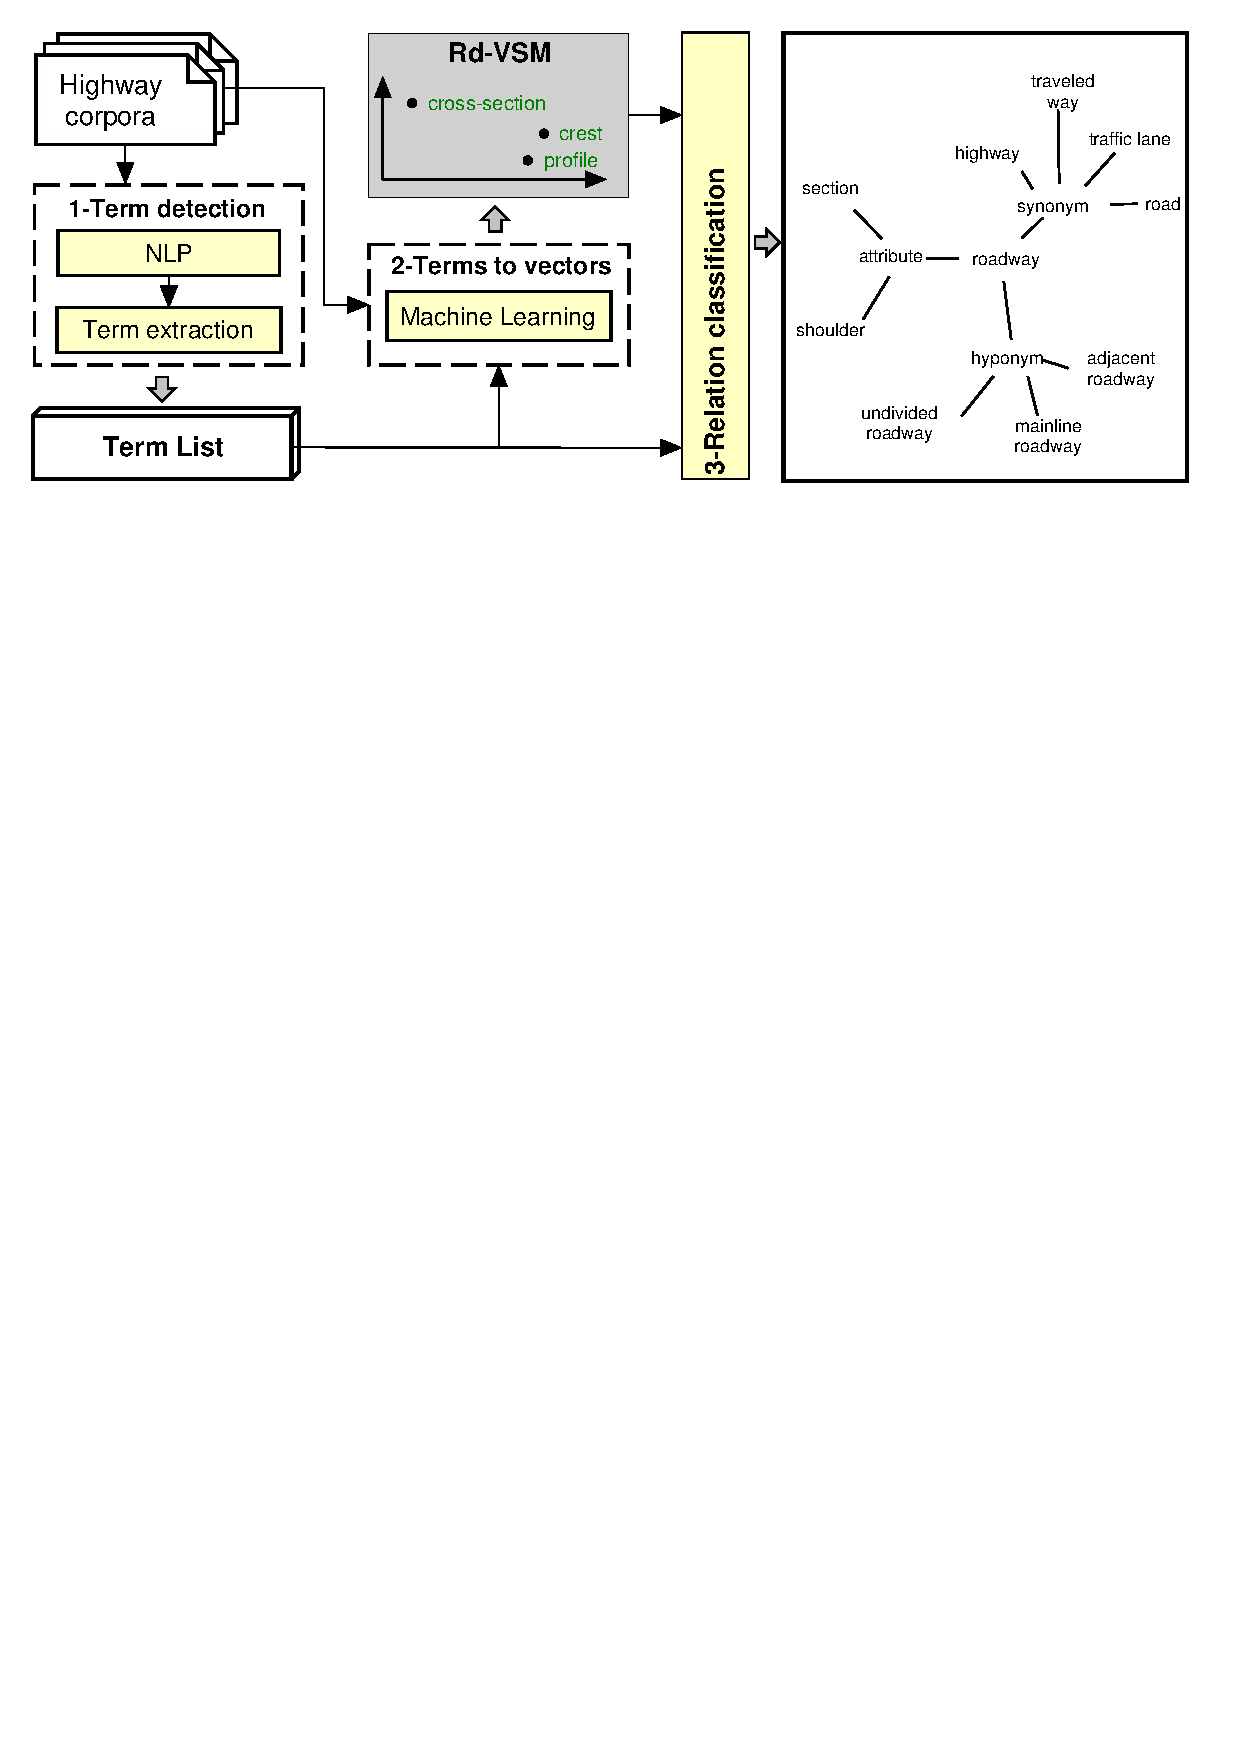
\includegraphics[width=0.95\textwidth]{Figure1_overview_methodology}
	\caption{Overview of the proposed methodology}
	\label{fig:framework}
\end{figure}
%
The ultimate goal of this research is to construct a machine-readable dictionary of technical terms, named InfraLex, for the infrastructure sector.  This research proposes a methodology for automated construction of the domain thesaurus using advanced Natural NLP techniques. 
\par
Figure \ref{fig:framework} presents an overview of the methodology proposed to develop InfraLex. The research framework is consisted of two major modules that are to: (1) train a highway term space model (H-VSM), and (2) develop an algorithm integrating H-VSM and linguistic patterns to construct InfraLex. The first module implements several basic NLP techniques (including tokenizing, POS tagging, etc.) and C-value \cite{frantzi20} method to extract highway related technical terms from a highway corpora. Skip-gram model, an unsupervised machine learning platform proposed by \cite{mikolov13a}, is then implemented to train the semantic similarity between technical terms. The model uses the unlabeled highway corpora as the training dataset. This training process transforms the identified terms into representation vectors in a coordinate space model named H-VSM.  Using this term vector space, the degree of similarity between technical terms can be determined; and based on that a list of the nearest terms for a given term can be obtained. In the second module, a computational algorithm is designed to classify the nearest lists resulted from the H-VSM into lexical groups by semantic relations such as synonymy, sibling, hypernymy, hyponymy and attribute. Specifically, the procedure followed to compile the InfraLex dictionary is comprised of the following steps which will be discussed in detail in the below sections.
\begin{itemize}
\item Collect highway technical documents to compose a domain corpus;
\item Extract multi-word terms from the highway corpus;
\item Prepare training dataset for training H-VSM;
\item Selecting training parameters and train H-VSM;
\item Design an algorithm to classify related terms into groups of lexical relations.
\end{itemize}

%
%TODO: The preliminary result is presented by. In this paper, the model is extended with larger training datasets and post-processing to reorganize terms in categories which improves the semantic data searching algorithm.
%\section{Highway term space model development} \label{sec:vector-space}
%
%introduction to the distributional vector model, fundamental theory,  the overall process to translate technical terms into vectors representations. the role of vector space allow measure the similarity between 
%TODO: This section presents the extension of the H-VSM developed by the authors' previous work with the extending of training datasets and post-processing of the vector space model.
%
\subsection{Data collection}
%how to collect data, how to clean data to get them readay for training model
%aim text folow remained, flow direction. bottom down, 
%remove heading (chapter, section, subsection), footnote, numerbing, bullets, hyperlink, url, 
As mentioned earlier, H-VSM was trained using a machine learning model which uses text corpus as the training data. A highway corpus was built upon the technical documents collected from multiple sources including textbooks, and highway engineering manuals from the Federal Department of Transportation (DOT) and 22 distinct State DOTs. The focus of this corpora is on the following three project phases: (1) design, (2) construction, and (3) asset management. Technical terms in a guidance document in the engineering field are organized in various formats such as plain text, tables, and equations. Since tables and equations are not yet supported by the state-of-the-art NLP techniques, they were removed from the text corpora. The final outcome of this phase is a plain text corpus consisting of 16 million words. This dataset is utilized to extract highway related technical terms which are then trained and converted into vectors.
%
\subsection{Multi-word terms extraction}
%
\begin{figure}[t]
	\centering
	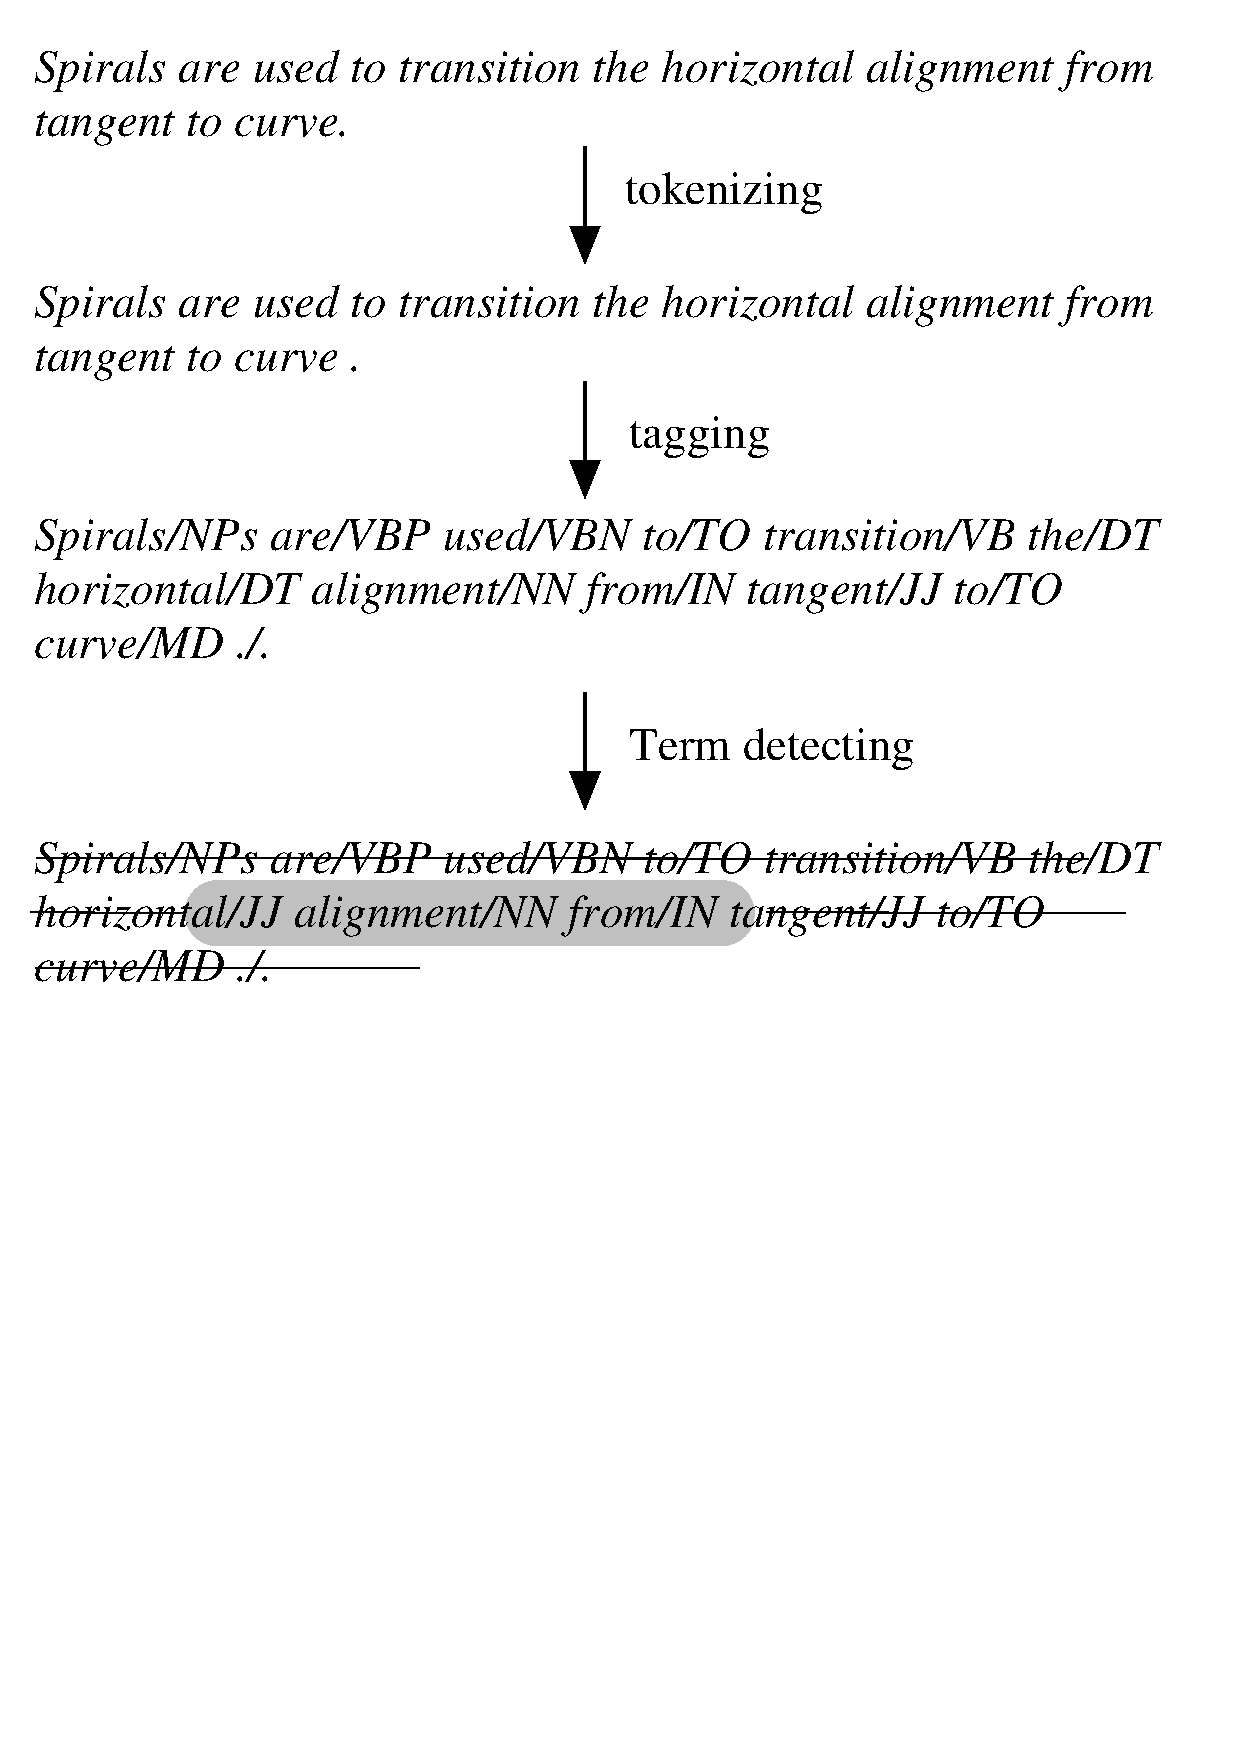
\includegraphics[width=0.45\textwidth]{Figure2_term_extraction}
	\caption{Linguistic processing procedure to detect technical terms}
	\label{fig:np_detect}
\end{figure}
%
A technical term can be a single word (e.g., roadway, lane, etc.) or be composed of multiple words (e.g., right of way, at grade intersection, etc.). The meaning of multi-word terms may not be directly interpreted from the meanings of their single words. In order for the Skip-gram model to learn the semantics of multi-word terms, every occurrence of multi-word terms in the corpus needs to be detected and replaced with connected blocks of word members so that they can be treated as single words. Figure \ref{fig:np_detect} presents the process of detecting technical terms from the set of highway technical documents. The process includes the following steps. 
\par
\begin{enumerate}
	\item \textbf{Word tokenizing:} In this step, the text corpus is broken down into individual units (also called tokens) using OpenNLP Tokenizer.
	\item \textbf{Part of Speed tagging:} The purpose of this step is to determine the POS tag (e.g., noun, adjective, verb, etc.) of each token.
	\item \textbf{Noun phrase detection:} Linguists argue that a technical term is either a noun (e.g., road) or a noun phrase (NP) (e.g., right of way) that frequently occurs in the domain text documents \cite{justeson95}. Thus, NPs are good multi-word term candidates. Table \ref{table:term_filter} presents the proposed extraction patterns which are modified from the filters suggested by \cite{justeson95} to extract NPs. The first two filters directly detect NPs that occur separately, and the third filter is to count for cases where multiple terms are written in conjunctions (e.g., 'vertical and horizontal alignment'). To extract NPs from a conjunction, an extra processing is applied to break it into individual NPs. For example, the conjunction 'vertical and horizontal alignment' will become 'vertical alignment' and 'horizontal alignment'. This division process determines the main part ('alignment') which is shared by two NPs and the dependent parts ('vertical' and 'horizontal'). This research uses Stanford Dependencies Parsing tool, which is able to analyze dependencies between sentiment units, to split conjunctions into separate phrases. 
	%
	\begin{table} [t]
		\caption{Term candidate filters}
		\label{table:term_filter}
		\centering
		\small
		\renewcommand{\arraystretch}{1.25}
		\begin{tabular}{l l}
			\hline
			\textbf{Pattern} & \textbf{Examples}\\
			\hline
			(Adj|N)*N		& road, roadway shoulder, vertical alignment\\
			(Adj|N)*N Prep (of/in) (Adj|N)*N	&	right of way, type of roadway\\
			(Adj|N)* 'and/or' (Adj|N)*N & vertical and horizontal alignment\\
			\hline
			\multicolumn{2}{l}{\textit{Note:} |, * respectively denotes 'and/or', and 'zero or more'.  } \\
			\hline
		\end{tabular}
		\normalsize
	\end{table}
	%
	\par
	In addition, in order to avoid the distinguishing between syntactic variants of the same term, for example 'roadway' and 'roadways', term variants will be normalized. The following are three types of syntactic variants and the proposed normalization methods. 
	\begin{itemize}
		\item \textbf{Type 1} - Plural forms, for example 'roadways' and 'roadway'. The Porter stemming algorithm [\cite{porter80}], which can allow for automated removal of suffixes, is applied on the corpus before extracting NPs.
		\item \textbf{Type 2} - Preposition noun phrases, for example 'roadway type' and 'type of roadway'. In order to normalize this type of variant, the form with preposition needs to be converted into the non-preposition form by removing the preposition and reverse the order of the remaining portions. For example, 'type of roadway' will become 'roadway type'.
		\item \textbf{Type 3} - Abbreviations, such as AADT. A linguistic rule-based method suggested by \cite{nenadic02} will be used to determine the full NP of an abbreviation. This method suggests the following abbreviation definition patterns: (1) left definition pattern - NP (Abbreviation), for example Annual Average Daily Traffic (AADT); and (2) right definition pattern - (Abbreviation) NP, for example (AADT) Annual Average Daily Traffic.
	\end{itemize}
	\item \textbf{Multi-word term candidate raking and selection:} Multi-word term definition varies between authors, and there is a lack of formal rules for defining multi-word term \cite{frantzi20}. There are a number of methods for estimating termhood (the degree that a linguistic unit is a domain-technical concept) such as TF-IDF  \cite{sparck72,salton88}, C-Value \cite{frantzi20}, Termex  \cite{sclano07}. These methods are based on occurrence frequencies of NPs in the corpus. Among these methods, Termex outperformed other methods on the Wikipedia corpus, and C-Value was the best on the GENIA medical corpus \cite{zhang08}. This result indicates that C-value method is more suitable for term extraction from a domain corpus rather than a generic corpus. For this reason, the C-value has been widely used to extract domain terms in the biomedical field \cite{ananiadou20}, \cite{lossio13}, and \cite{nenadic02}. Since the corpus used in this study was mainly collected from technical domain documents, thus C-value would be the most suitable for termhood determination. The C-value measure, as formulated in Equation \ref{eq:cvalue}, suggests that the longer a NP is, the more likely that is a term; and the more frequently it appears in the domain corpus, the more likely it will be a domain term.
	% 
	\begin{equation}
	C-value(a)=
	\begin{cases}
	log_2|a|.f(a), & \text{if a is not nested} \\
	log_2|a|(f(a)-\frac{1}{P(T_a)}\sum_{b\in T_a} f(b)), & \text{otherwise}
	\end{cases}
	\label{eq:cvalue}
	\end{equation}
	%
	Where:
	\begin{description}
		\item[a] is a candidate noun phrase
		\item[f] is the frequency of a in the corpus
		\item[Ta] is the set of extracted noun phrases that contains a
		\item[P(Ta)] is the number of these candidate terms.
	\end{description}
\end{enumerate}
%
\par
The process above results in a dataset containing detected terms along with their termhood scores. These terms are ordered by C-value, and the ones that have negative C-values are discarded. 
\par
To remove non-terms from the term list, a manual evaluation process was conducted. Table \ref{table:term_evaluation} shows the evaluation result for 5 examples of the extracted terms. The longer the list is, the more effort required for the evaluation process. Since term extraction is based on frequency, the size of term list will be affected if a threshold of frequency is used. With the threshold of 2, the list consists of 112,024  terms. The list size drops to 8,922 when a threshold of 50 is used. Manually reviewing such a long list is still a challenging task. To minimize human force, the list was evaluated at several ranges of C-values. Precision, which represents the percentage of real terms in each group, is presented in Figure \ref{fig:term_precision}. As shown in the figure, precision values are relative low for groups with c-values less than 70. To balance between human cost and precision of the final term list, this research applied the manual review on all of the automatically extracted terms below the c-value threshold of 70.
%To calculate the recall value, expert is required to final all true terms from the corpus \cite{frantzi20}. with the large corpus in this research, it is impossible to do this task. 
%
\begin{table} [t]
	\caption{Examples of extracted terms and evaluation}
	\label{table:term_evaluation}
	\centering
	\small
	\renewcommand{\arraystretch}{1.25}
	\begin{tabular}{l l l}
		\hline
		\textbf{Term} & \textbf{Termhood} & \textbf{real term?}\\
		\hline
		sight distance		& 9435.314 & yes\\
		design speed & 9052.556 & yes \\
		additional information & 1829.0 & no\\
		typical section & 1801.0  & yes\\
		basis of payment & 1762.478 & no\\
		\hline
	\end{tabular}
	
	\normalsize
\end{table}

\begin{figure}[t]
	\centering
	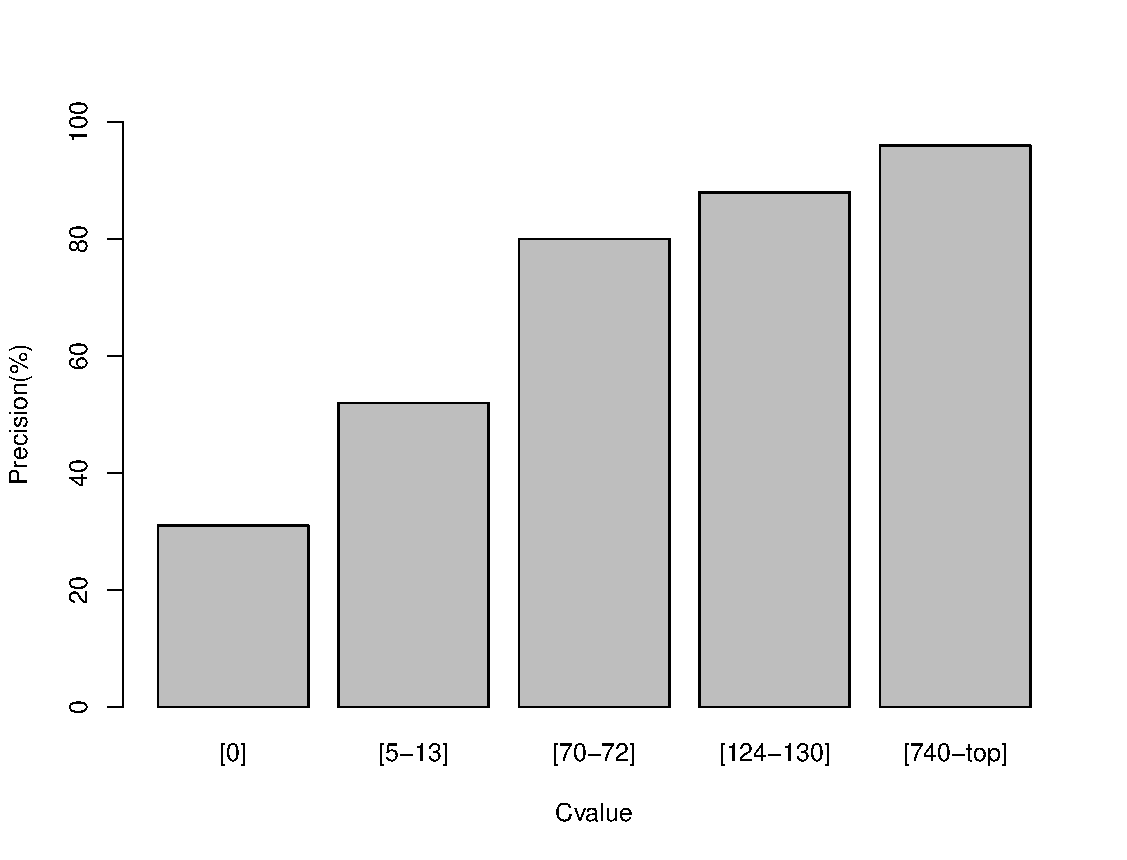
\includegraphics[width=0.5\textwidth]{Figure3_term_precision}
	\caption{Precision of term extraction}
	\label{fig:term_precision}
\end{figure}

\subsection{Training dataset preparation}
The highway text corpora collected serves as the source of training dataset for developing the semantic similarity model. The Skip-Gram model requires a set of training data in which the input data is a linguistic unit (word or term), and the output data is a set of context words. In order to collect this training dataset, the unannotated text corpora will be scanned to collect instances of terms and their corresponding context words. Each occurrence of a word will correspondingly generate a data point in the training dataset.
\par
Before collecting the training dataset, an additional step is needed to handle the issue related to multi-word terms. Since document scanning is on a word-by-word basis, the corpus must be adjusted so that multi-word terms can be treated like single words. To fulfill that requirement, every occurrence of a multi-word term in the corpus is replaced with a single unit that is compiled by connecting all individual words. For instance, 'vertical alignment' becomes 'vertical-alignment'.
\par
The number of context words to be collected is dependent on the window size that limits how many words to the left and the right of the target word. In the example sentence below, the context of the term 'roadway' with the context window size of 10 will be the following word set \{bike, lane, width, on, a, width, no, curb, gutter\}. Any context word that is in the stop list (the list contains frequent words in English such as 'a', 'an', 'the' that have little meaning) will be neglected in the context set.
%
\begin{center}
	"The minimum [bike lane width on a \underline{roadway} with no curb and gutter] is 4 feet."
\end{center}
%
\subsection{Semantic similarity training}
%word2vec, brief introduction about word2vec
%skip-gram model
%how to modify the method of selecting conext words
%java program
%
\begin{figure}[t]
	\centering
	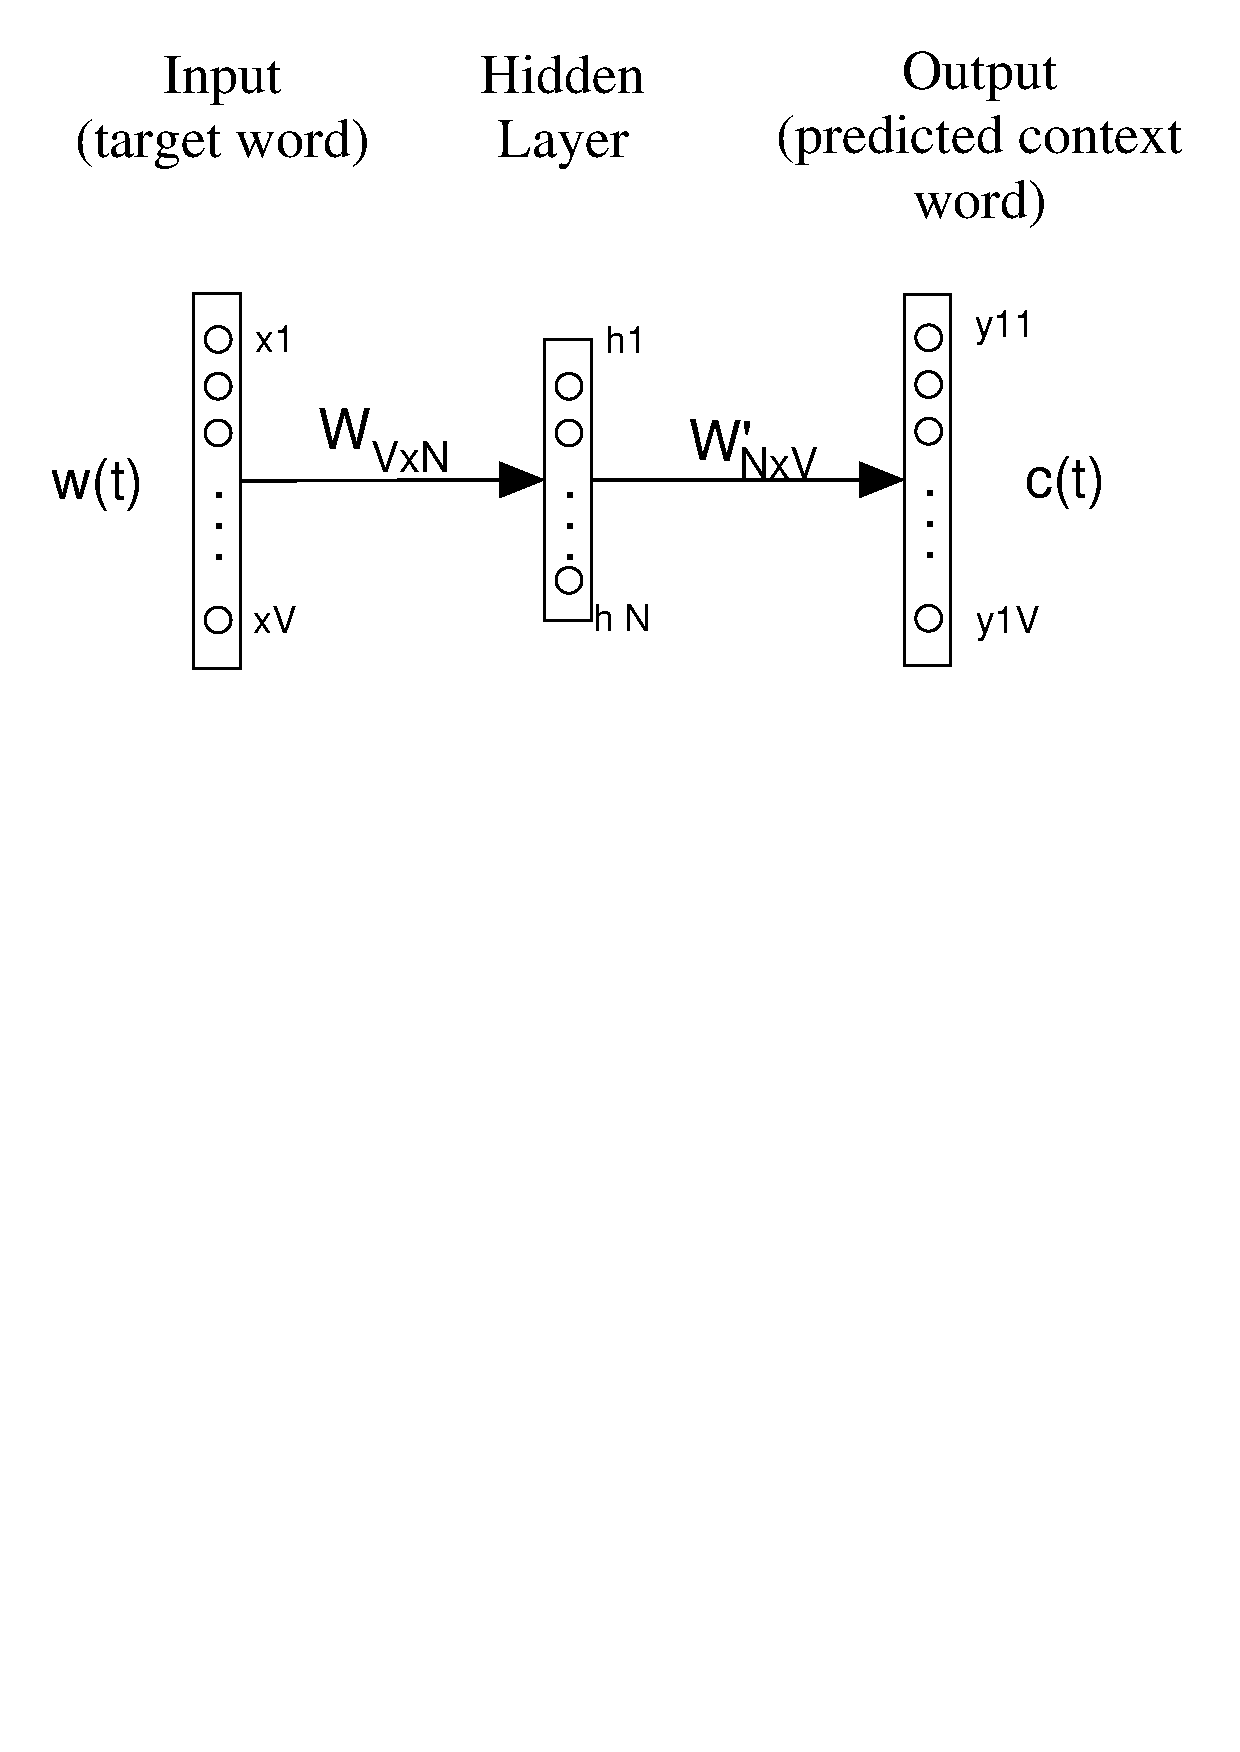
\includegraphics[width=0.45\textwidth]{Figure4_skip-gram-model}
	\caption{Skip-gram model}
	\label{fig:skip-gram}
\end{figure}
%
The semantic similarity will be trained using the word2vec module in the Apache Spark MLlib package \cite{apache16}, an emerging open-source engine, developed based on the Skip-gram neural network model \cite{mikolov13a}. The model includes three major parameters that are frequency threshold, hidden layer size and window size (see Table \ref{table:nn-parameters}). To eliminate data points with low frequency of occurrence that are unlikely to be technical terms, word2vec includes the parameter of \textit{frequency threshold}. Any vocabulary with the rate lower than the limit will be ignored. Radim Rehurek, a machine learning consultant company, suggests a range of (0-100) depending on the data set size. Setting this parameter high will enhance the accuracy, but many technical terms will be out of vocabulary. A preliminary study based on the preliminary corpus with only several millions of words shows that with the frequency of 20, there are very few non-technical terms involved in the training dataset. Hence, with the larger dataset to be collected, this parameter can be higher and up to around 50. The second important parameter is \textit{layer size} which determines the number of nodes in the hidden layer. This parameter highly affects the training accuracy and processing time. A larger layer size is better in terms of accuracy, but this will be paid off by the running time. Since this research aims to develop a model that can be used for other information retrieval research, the accuracy is the first priority. This parameter is suggested to be in the range of 100-500. The final major parameter is \textit{context window size}. Google suggests the size of 10 for the Skip-gram model. These parameters are subject to be changed so that the best model can be achieved. The effects of these parameters on the model performance are discussed in Section \ref{sec:eval_infralex}.
%
\begin{table} [t]
	\caption{Skip-gram model parameters}
	\label{table:nn-parameters}
	\centering
	\small
	\renewcommand{\arraystretch}{1.25}
	\begin{tabular}{l l}
		\hline
		\textbf{Parameter} & \textbf{Value}\\
		\hline
		Frequency threshold & 50-100\\
		Hidden layer size		&	100-500\\
		Context window size	&	5,10,15\\
		\hline
	\end{tabular}
	\normalsize
\end{table}
%
\par
Figure \ref{fig:hvsm} presents the term space model developed from the training process when the parameters are set 50, 300 and 10 respectively. In this model, each technical term collected from technical documents is represented as a vector in a high dimensional space; and the distance between terms represents semantic similarity. H-VSM is consisted of more than 6,000 technical keywords. Since the vector space is a multi-dimensional space in accordance with the size of the hidden layer. In order to present the space in 2D graph, PCA (Principle Component Analysis) was used to reduce the size to 2 dimensions. 
\par
The similarity between terms can be measured by the angle between two word representation vectors (Equation \ref{equ:cosin_sim}) or the distance between two word points (Equation \ref{equ:dis_sim}). Table \ref{table:nearest_example} shows an example of a ranked list of near terms obtained from the H-VSM model in order of similarity score.
%
\begin{figure}[t]
	\centering
	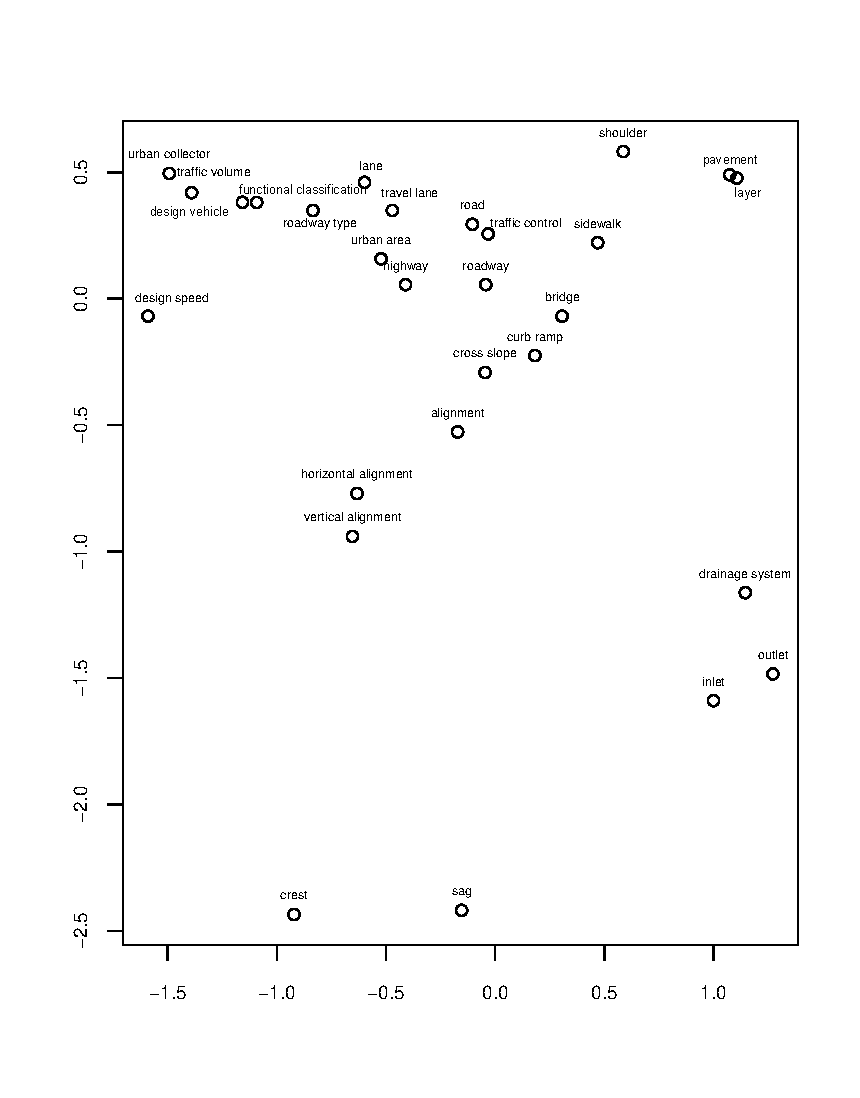
\includegraphics[width=0.45\textwidth]{Figure5_hvsm_space}
	\caption{Highway term space model (H-VSM)}
	\label{fig:hvsm}
\end{figure}
%
\begin{equation}
\label{equ:cosin_sim}
cosine\_similarity = \frac{A.B}{||A||.||B||}
\end{equation}

\begin{equation}
\label{equ:dis_sim}
dis\_similarity =\sqrt{(xA_1-xB_1)^2+(xA_2-xB_2)^2+...+(xA_n-xB_n)^2}
\end{equation}

Where: n is the hidden layer size.
%
\begin{table} [t]
	\caption{Examples of top nearest terms}
	\label{table:nearest_example}
	\centering
	\small
	\renewcommand{\arraystretch}{1.25}
	\begin{tabular}{l l l  l}
		\hline
		\textbf{Term} & \textbf{Nearests} & \textbf{Cosine} &\textbf{Rank}\\
		\hline
		roadway			& highway & 0.588 & 1\\
		& traveled-way & 0.583 & 2\\
		& roadway-section & 0.577 & 3\\
		& road & 0.533 & 4\\
		& traffic-lane & 0.524 &5\\
		& separating & 0.522 &6\\
		& adjacent-roadway & 0.519 & 7\\
		& travel-way & 0.517 & 8\\
		& entire-roadway & 0.513 & 9\\
		& ...&...& ...\\
		& roadway-shoulder & 0.505 & 12\\
		& roadway-cross-section & 0.491 & 18\\
		& undivided & 0.452 & 37\\
		& mainline-roadway & 0.450 & 42\\
		\hline
	\end{tabular}
	\normalsize
\end{table}

\subsection{Highway lexicon construction}
The purpose of this module is to construct a lexicon which is also known as lightweight ontology. A knowledge base typically includes terms and relations. The core relations of a lexicon can be classified into the following types: synonym (meaning equivalence), hypernym-hyponym (also known as IS-A or parent-child relation), attribute (concept property), and association (e.g. part-of) \cite{jiang97,lee13}. Two terms relate each other through these semantic relation would have a high similarity score. Therefore, the top nearest terms resulted from H-VSM would be a great starting point for detecting relations between technical terms. Table \ref{table:nearest_example} illustrates a list of nearest terms of the term 'roadway'. In this list, true synonyms are highway (1), traveled-way (2) or road(4); attributes include roadway-section (3), roadway-shoulder (12); and adjacent-roadway (7) and undivided (37) are hyponyms which showing different types of roadway.
\par
The specific objective of this task is to detect relations and based on that rearrange the nearest terms obtained from the H-VSM model. Algorithm \ref{alg:term_class} shows the design pseudo code for classifying the nearest terms of a given target term. The algorithm utilizes linguistic rules and clustering analysis to reorganize the nearest list into the following three groups: (1) attribute, (2) hyponym, and (3) synonym/sibling and other functional relations. The algorithm firstly detects terms for the first two categories using linguistic patterns. The filter rules to detect these relations are presented in Table \ref{table:attribute_pattern}. For a multi-word term matching pattern 1, we can infer that Noun1 is an attribute of concept Noun2; and Noun2 is an attribute of Noun1 in the pattern 2. Pattern 3 is for detecting hyponyms where the matched NP is a hyponym of Noun2 concept.  The remained nearest words will fall into the third group. However, some of them have far or even no relation with the target word. In order to address this issue, this research employed the K-mean clustering algorithm \cite{macqueen67} to split the remained list into three distinct layers based on the similarity score. The terms in the last group are unlikely to be a synonym or sibling and are removed from the nearest list. The output of the proposed algorithm is a list of classified nearest terms. Table \ref{table:term_clustering} shows one example for the output retrieved from the algorithm. 
%In contrast, since synonym recognition is well known as the process of evaluating the sharing of common attributes, hypernyms, and hyponyms, this process will rely on the results from the detection of other relations. This task will first detect the following relations (hypernyms, hyponyms and attributes) and then use them as features to find synonyms.
%
\begin{algorithm}[h]
	
	\caption{Near term classification algorithm}\label{alg:term_class}
	\begin{algorithmic}[1]
		\State \textbf{Inputs}: term \textit{t}, list of nearest terms \textit{N}, full list of terms \textit{F}
		\State \textbf{Output:}: Classified list of terms \textit{C}
		\Procedure{Term classification procedure}{}
		%\State $\textit{n} \gets \text{size of }\textit{W}$
		%\State $\textit{m} \gets \text{size of }\textit{T}$
		\State $\textit{Att} \gets \text{list of attributes}$
		\State $\textit{Hyp} \gets \text{list of hyponyms}$
		\State $\textit{Syn} \gets \text{list of synonyms}$
		\State $\textit{w} \gets \textit{null}$
		\ForAll {$n \in N$}
		\If {$n$ contains \textit{t}}
		\State $w \gets n$
		
		\Else
		\ForAll {$f \in F$}
		\If {$f$ contains both $n$ and \textit{t}}
		\State $w \gets f$	
		\State Break for
		
		\EndIf
		\EndFor
		\EndIf
		\EndFor
		\If {$w$ matches \textit{Attribute pattern}}
		\State add $w$ to \textit{Att}
		\ElsIf {$w$ matches \textit{Hyponym pattern}}
		\State add $w$ to \textit{Hyp}
		\Else
		\State add $w$ to \textit{Syn}
		\EndIf
		\State Cluster \textit{Syn} and discard low relevant terms
		
		\EndProcedure
	\end{algorithmic}
\end{algorithm}
%
%\subsection{Attribute and hyponym patterns}
%
\begin{table} [t]
	\caption{Patters to extract attributes and hyponyms}
	\label{table:attribute_pattern}
	\centering
	\small
	\renewcommand{\arraystretch}{1.25}
	\begin{tabular}{l l l}
		\hline
		\textbf{Relation} & \textbf{Pattern} & \textbf{Example}\\
		\hline
		Attribute &	Noun1 of Noun2 & the width of the road\\
		& Noun1 Noun2	&	road width, project cost\\
		Hypernym-hyponym & Noun1 Noun2 & vertical alignment isA alignment\\
		\hline
	\end{tabular}
	\normalsize
\end{table}
%
%After the candidate list is refined, the frequency of occurrence for each candidate will then be used to compute the degree that term 'a' is an attribute of concept 'c'. If 'a' is a typical attribute of 'c', it should frequently occur in the corpus. Each concept 'c' will correspondingly have a list of attribute candidates (called list A) and their frequency of occurrences. The likelihood that 'a' is an attribute of concept 'c' is estimated using the normalized probability formula (see Equation \ref{eq:attribute}). The attribute candidates for each concept will be ranked by the likelihood measure and the top list over a threshold value will be accepted as typical attributes. 
%\begin{equation}
%P(a|c)=\frac{n(c,a)}{\sum_{a* \in A} n(c,a)}
%\label{eq:attribute}
%\end{equation}
%\subsection{Synonym/sibling and functional relation recognition}

%
\begin{table} [t]
	\caption{Examples of top nearest terms}
	\label{table:term_clustering}
	\centering
	\small
	\renewcommand{\arraystretch}{1.25}
	\begin{tabular}{l l l l l}
		\hline
		\textbf{Term}	&\textbf{Relation Group}	& \textbf{Nearests} & \textbf{Cosine} & \textbf{Rank}\\
		roadway			&Synonym					& highway & 0.588 & 1\\
		&							& traveled-way & 0.583 & 2\\
		&							& road & 0.533 & 4\\						
		&							& traffic-lane & 0.524 &5\\ 						
		&							& travel-way & 0.517 & 8\\  \cmidrule{2-5}
		&Attribute					& separating & 0.522 &6\\
		&							& roadway-section & 0.577 & 3\\						
		&							& roadway-shoulder & 0.505 & 12\\
		&							& roadway-cross-section & 0.491 & 18\\\cmidrule{2-5}						
		&Hyponym					& adjacent-roadway & 0.519 & 7\\
		&							& entire-roadway & 0.513 & 9\\
		&							& undivided & 0.452 & 37\\
		&							& mainline-roadway & 0.450 & 42\\
		\hline
	\end{tabular}
	\normalsize
\end{table}


\section{Performance evaluation} \label{sec:eval_infralex}
%evaluation method
This section presents a performance evaluation of InfraLex on the ability to identify synonyms. In this experiment, a gold standard  is used. The gold standard is consisting 70 sets of synonyms (both single and multi-word terms) which were examined and extracted from a Wikipedia transportation glossary \cite{wikipedia16}. This glossary provides plain text explanation for each term and their synonyms. The automatically identified synonym which is the top nearest word of the synonym/sibling lexical group was compared with the true synonym in the gold standard dataset. The results are evaluated using the following three measures including recall, precision and f-measure.
%
\begin{align} 
&Recall = \frac{\text{number of correctly matched concepts}}{\text{total concepts}}  \\ 
&Precision = \frac{\text{number of correctly matched concepts}}{\text{total matched concepts}}  \\
&F-measure = \frac{2.Precision.Recall}{Precision+Recall}
\end{align}
%results
\begin{table} [b] 
	\caption{Effects of training parameters on performance of synonym matching}
	\label{table:eval_syn_par_effect}
	\centering
	\small
	\renewcommand{\arraystretch}{1.25}
	\begin{tabular}{l l l l l }
		\hline
		\hline
		\textbf{Parameter} & \textbf{Model} & \textbf{Precision (\%)}  & \textbf{Recall(\%)} & \textbf{F (\%)}\\
		\hline
		Baseline	&	50-100-5	&79		&53		&63\\
		\hline
		\textbf{Window size}	&\textbf{50-100-\underline{10}}	&\textbf{81}		&\textbf{54}		&\textbf{65}\\
		&50-100-\underline{15}	&81		&54		&65\\
		\hline		
		Frequency threshold	&\underline{75}-100-5	&74		&50		&60\\
		&\underline{100}-100-5	&77		&51		&62\\
		\hline
		Hidden layer size	&50-\underline{200}-5	&79		&53		&63\\
		\hline
		\hline
	\end{tabular}
	\normalsize
\end{table}
\par
%synonym matching peformance result
Table \ref{table:eval_syn_par_effect} shows the performance with different training model settings. The parameters of the baseline model are 50, 100 and 5 respectively for frequency threshold, hidden layer size and window size. We changed these parameters one by one and remained the other ones to evaluate their effects to the model performance. As presented in the table, the increase of window size to 10 or 15 resulted in the best model which have precision of 81\% and an F-measure of 65\%. The change of other parameters did not improve the performance. Especially, the increase of frequency threshold has negative impact. 
%compared to the previous publication by the authors, this algorithm has been improved with significantly higher accuracy. the post-processing is one reason for the out-performance of the proposed method.  
%
%result
\begin{table} [b] 
	\caption{Comparison of synonym matching performance between Wordnet and InfraLex}
	\label{table:eval_syn_vs_Wordnet}
	\centering
	\small
	\renewcommand{\arraystretch}{1.25}
	\begin{tabular}{l l l l }
		\hline
		\hline
		\textbf{Lexicon} & \textbf{Precision (\%)}  & \textbf{Recall(\%)} & \textbf{F (\%)}\\
		\hline
		Wordnet	&76 	&40 	&52\\	
		\textbf{InfraLex} &\textbf{81}	&\textbf{54}		&\textbf{65}\\	
		\hline
		\hline
	\end{tabular}
	\normalsize
\end{table}
\par
Table \ref{table:eval_syn_vs_Wordnet} presents the comparison of performance between InfraLex (with 50-100-10 settings) and Wordnet. As shown, InfraLex outperformed Wordnet in all aspects, and the combined F-measure is significantly improved (65\% compared to 52\%). The biggest contribution to the improvement of the overall F-measure is the recall value which represents a better coverage of domain vocabulary of InfraLex. 
%attribute  hyponyms and attributes. finding performance
%for attribute and hyponym only precision is determined. to determine the recall require of all possible true attributes for a concept which is challenging and unrealistic task, this research evaluate the accuracy of the extracted attributes. this largely depend on the size and the variety of discipiline covered in the corpus. select of one in each set of synonyms in the gold standard and  humam evaluate attribute and non-attribute. the performance in measure using Equation which represent the percentage of correctly extracted attribute/hyponym. 

%
\section{Discussions} \label{sec:dis}
%limitation and potential direction for improvement
The current study has several limitations that may be the reason for the low overall performance. Firstly, the highway corpus is still relatively small with only 160 million words, compared to corpus size in other domain. Since the recall value largely depends on the corpus size, the expansion of the highway corpus would enable more technical terms to be covered in InfraLex. Future research is needed to enhance the performance of InfraLex by enlarging the data training set in both size and the number of disciplines involved throughout the life cycle of a highway project. Another work that potentially improve the model performance is to distinguish synonym and sibling which still in the same group in the proposed InfraLex. When these two lexical relations are separated, the possibility to recognize a wrong synonym will be reduced; and consequently, the precision value would be enhanced.
%potential application
\par
The lexicon dataset developed in this study is expected to become an underlying resource for a variety of NLP related studies in the civil infrastructure domains. InfraLex would serve as a machine-readable dictionary of domain technical terms. NLP based platforms can utilize this resource for word sense analysis which is crucial for text mining to extract meaningful information from text documents, information retrieval, or natural language based human-machine interaction. Some specific examples of these potential applications are as follows. Firstly information retrieval systems can use the semantic relations provided by InfraLex to classify project documents by topic. Secondly, questionnaire designers can utilize InfraLex to search for synonyms so that appropriate terms can be selected in accordance with each group of potential respondents which may be from multiple disciplines or regions. Another application is that query systems to extract data from 3D engineered models would be able to find alternative ways to query data when users' keywords do not match any entity in the database. Since users have different ways and keywords to query data, the ability to recognize synonyms and related concepts of a query system would provide flexibility to the end user. Also, the developed InfraLex would enable the matching data items such as (e.g., cost, productivity, etc.) when integrating data from distinct departments or states. Last but not least, this study is expected to fundamentally transform the way human interacts with machine. Instead of using computer languages, the end user can use natural language to communicate with computer systems.
\par
%
\section{Conclusions} \label{sec:conclns3} 
Data manipulation and retrieval from multiple sources is a challenging task due to the inconsistency of data format and terminology. The contribution of this study is a digital lexicon of highway related technical terms (named InfraLex) which can enable a computer to understand semantic meanings of terms.  This research employs advanced NLP techniques to extract technical terms from a highway text corpus which is consisted of 16 million words built on a collection of design manuals from 22 State DOTs across the U.S. Machine learning was used to train the semantic similarity between technical terms. An algorithm was designed to classify the nearest terms resulted from the semantic similarity model into distinct groups according to their lexical relationships. This algorithm was employed to develop the InfraLex database. 
\par
The developed lexicon has been evaluated by comparing the resulted obtained from the computational model and a man-crafted gold standard. The result shows an accuracy of over 80 percent.  The best model is associated with the training parameters of 50, 100 and 10 respectively for frequency threshold, hidden layer size, and window size. Although significant improvement is shown in comparison with the existing thesaurus databases, the overall performance is relative low. This may be due to the size of the training data. Future research will be conducted to expand the highway corpus to further disciplines such as asset management, and transportation operation. 
\par
The research opens a new gate for computational tools regarding natural language processing in the highway sectors. InfraLex would enable computer systems to understand terms and consequently transform the way human interacts with computer by allowing users to use natural language. 

\bibliography{mybib}
%\bibliography{2nd_paper_bib}
%
%
\end{document}

